\chapter{Results}

The results section delves into the performance differences between static and dynamic action discovery methods across three key aspects: startup time, build duration, and memory usage during startup. Each subsequent section provides specific findings, illustrating how varying the number of controllers impacts these metrics and revealing the comparative performance implications of the two action discovery approaches.

\section{Startup Time}

Figure \ref{fig:dynamic-startup-100} illustrates the startup time for a small application comprising 100 controllers using the existing dynamic action discovery. An observable initial slowdown is noted, with the first run beginning around 21ms and gradually decreasing to around 18.5ms over 200 iterations. However, subsequent runs display a more consistent startup duration ranging between 10 and 11 milliseconds. Overall, the mean startup time of the application employing dynamic action discovery averages 12.55 milliseconds, with an error margin of 0.47 and a standard deviation of 3.95.

\begin{figure}[H]
\centering
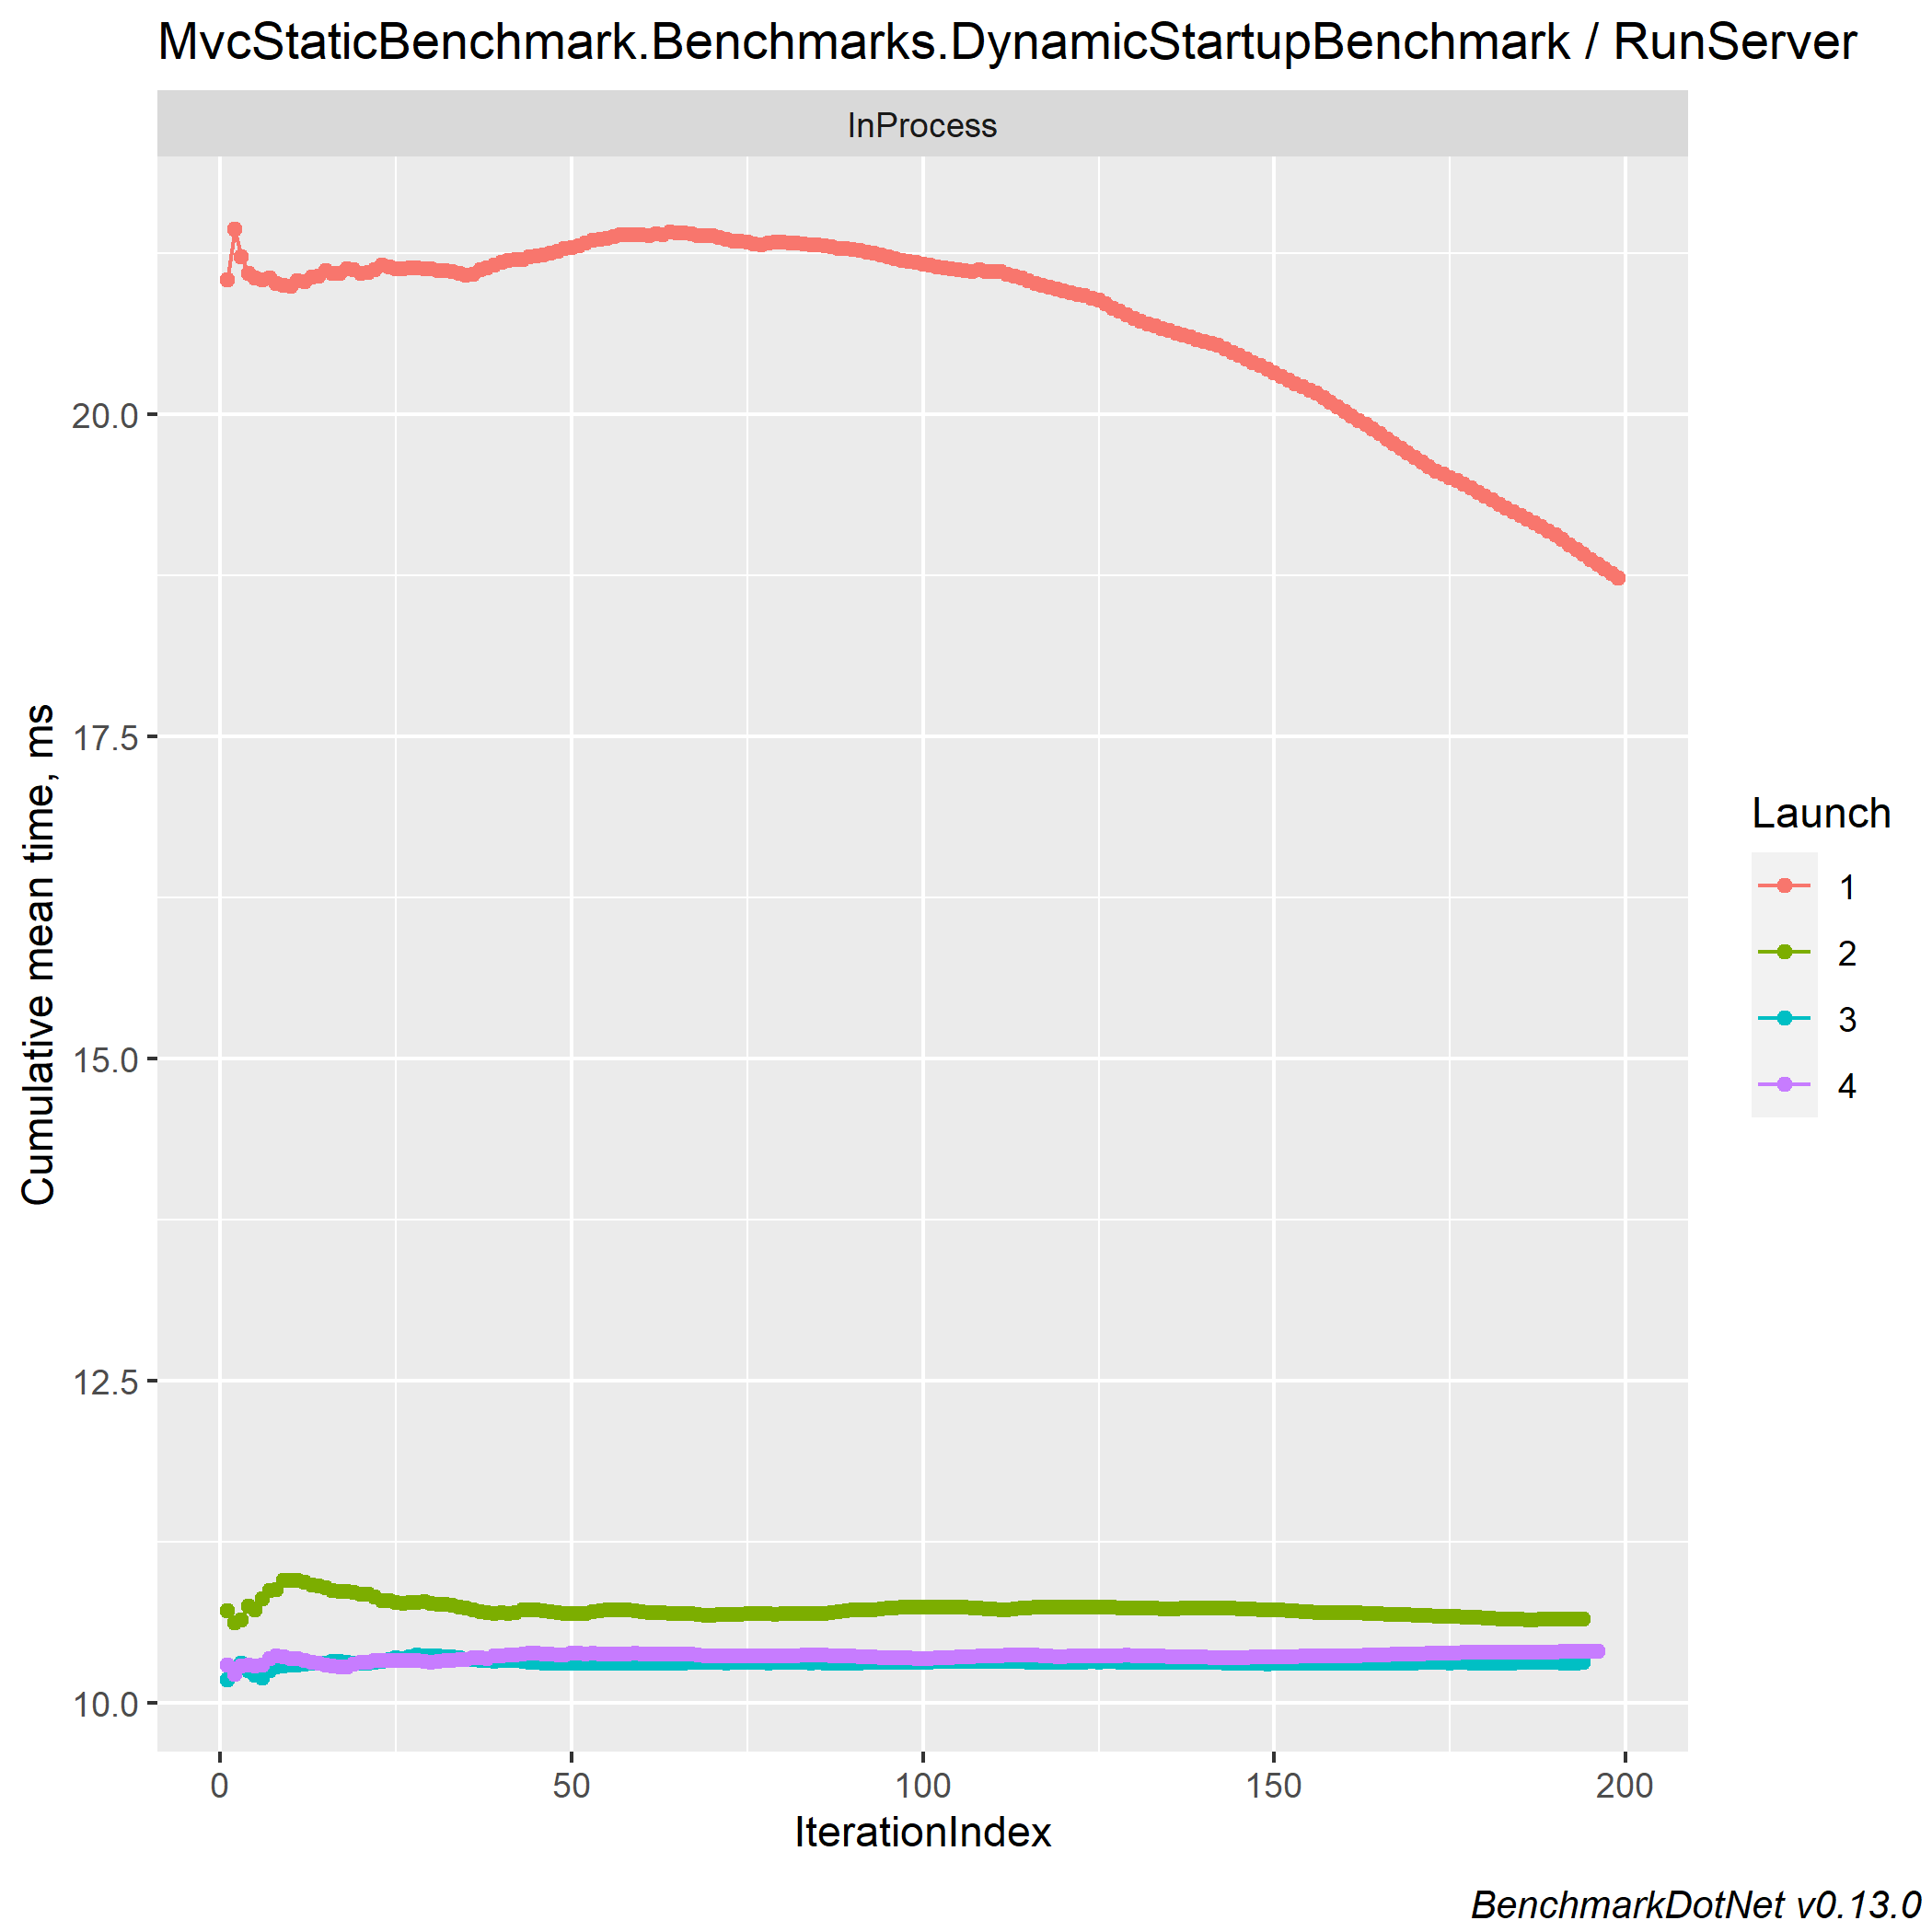
\includegraphics[width=0.8\textwidth]{graphics/MvcStaticBenchmark.Benchmarks.DynamicStartupBenchmark-RunServer-cummean.png}
\caption{Average startup time of an application using dynamic action discovery with 100 controllers}
\label{fig:dynamic-startup-100}
\end{figure}

In contrast, Figure \ref{fig:static-startup-100} presents the same application employing static action discovery. Here, the first two runs average around 6.5 milliseconds, while the last two runs maintain a consistent speed of approximately 3 milliseconds. This setup results in a mean startup time of 4.68 milliseconds, an error margin of 0.19, and a standard deviation of 1.59.

\begin{figure}[H]
\centering
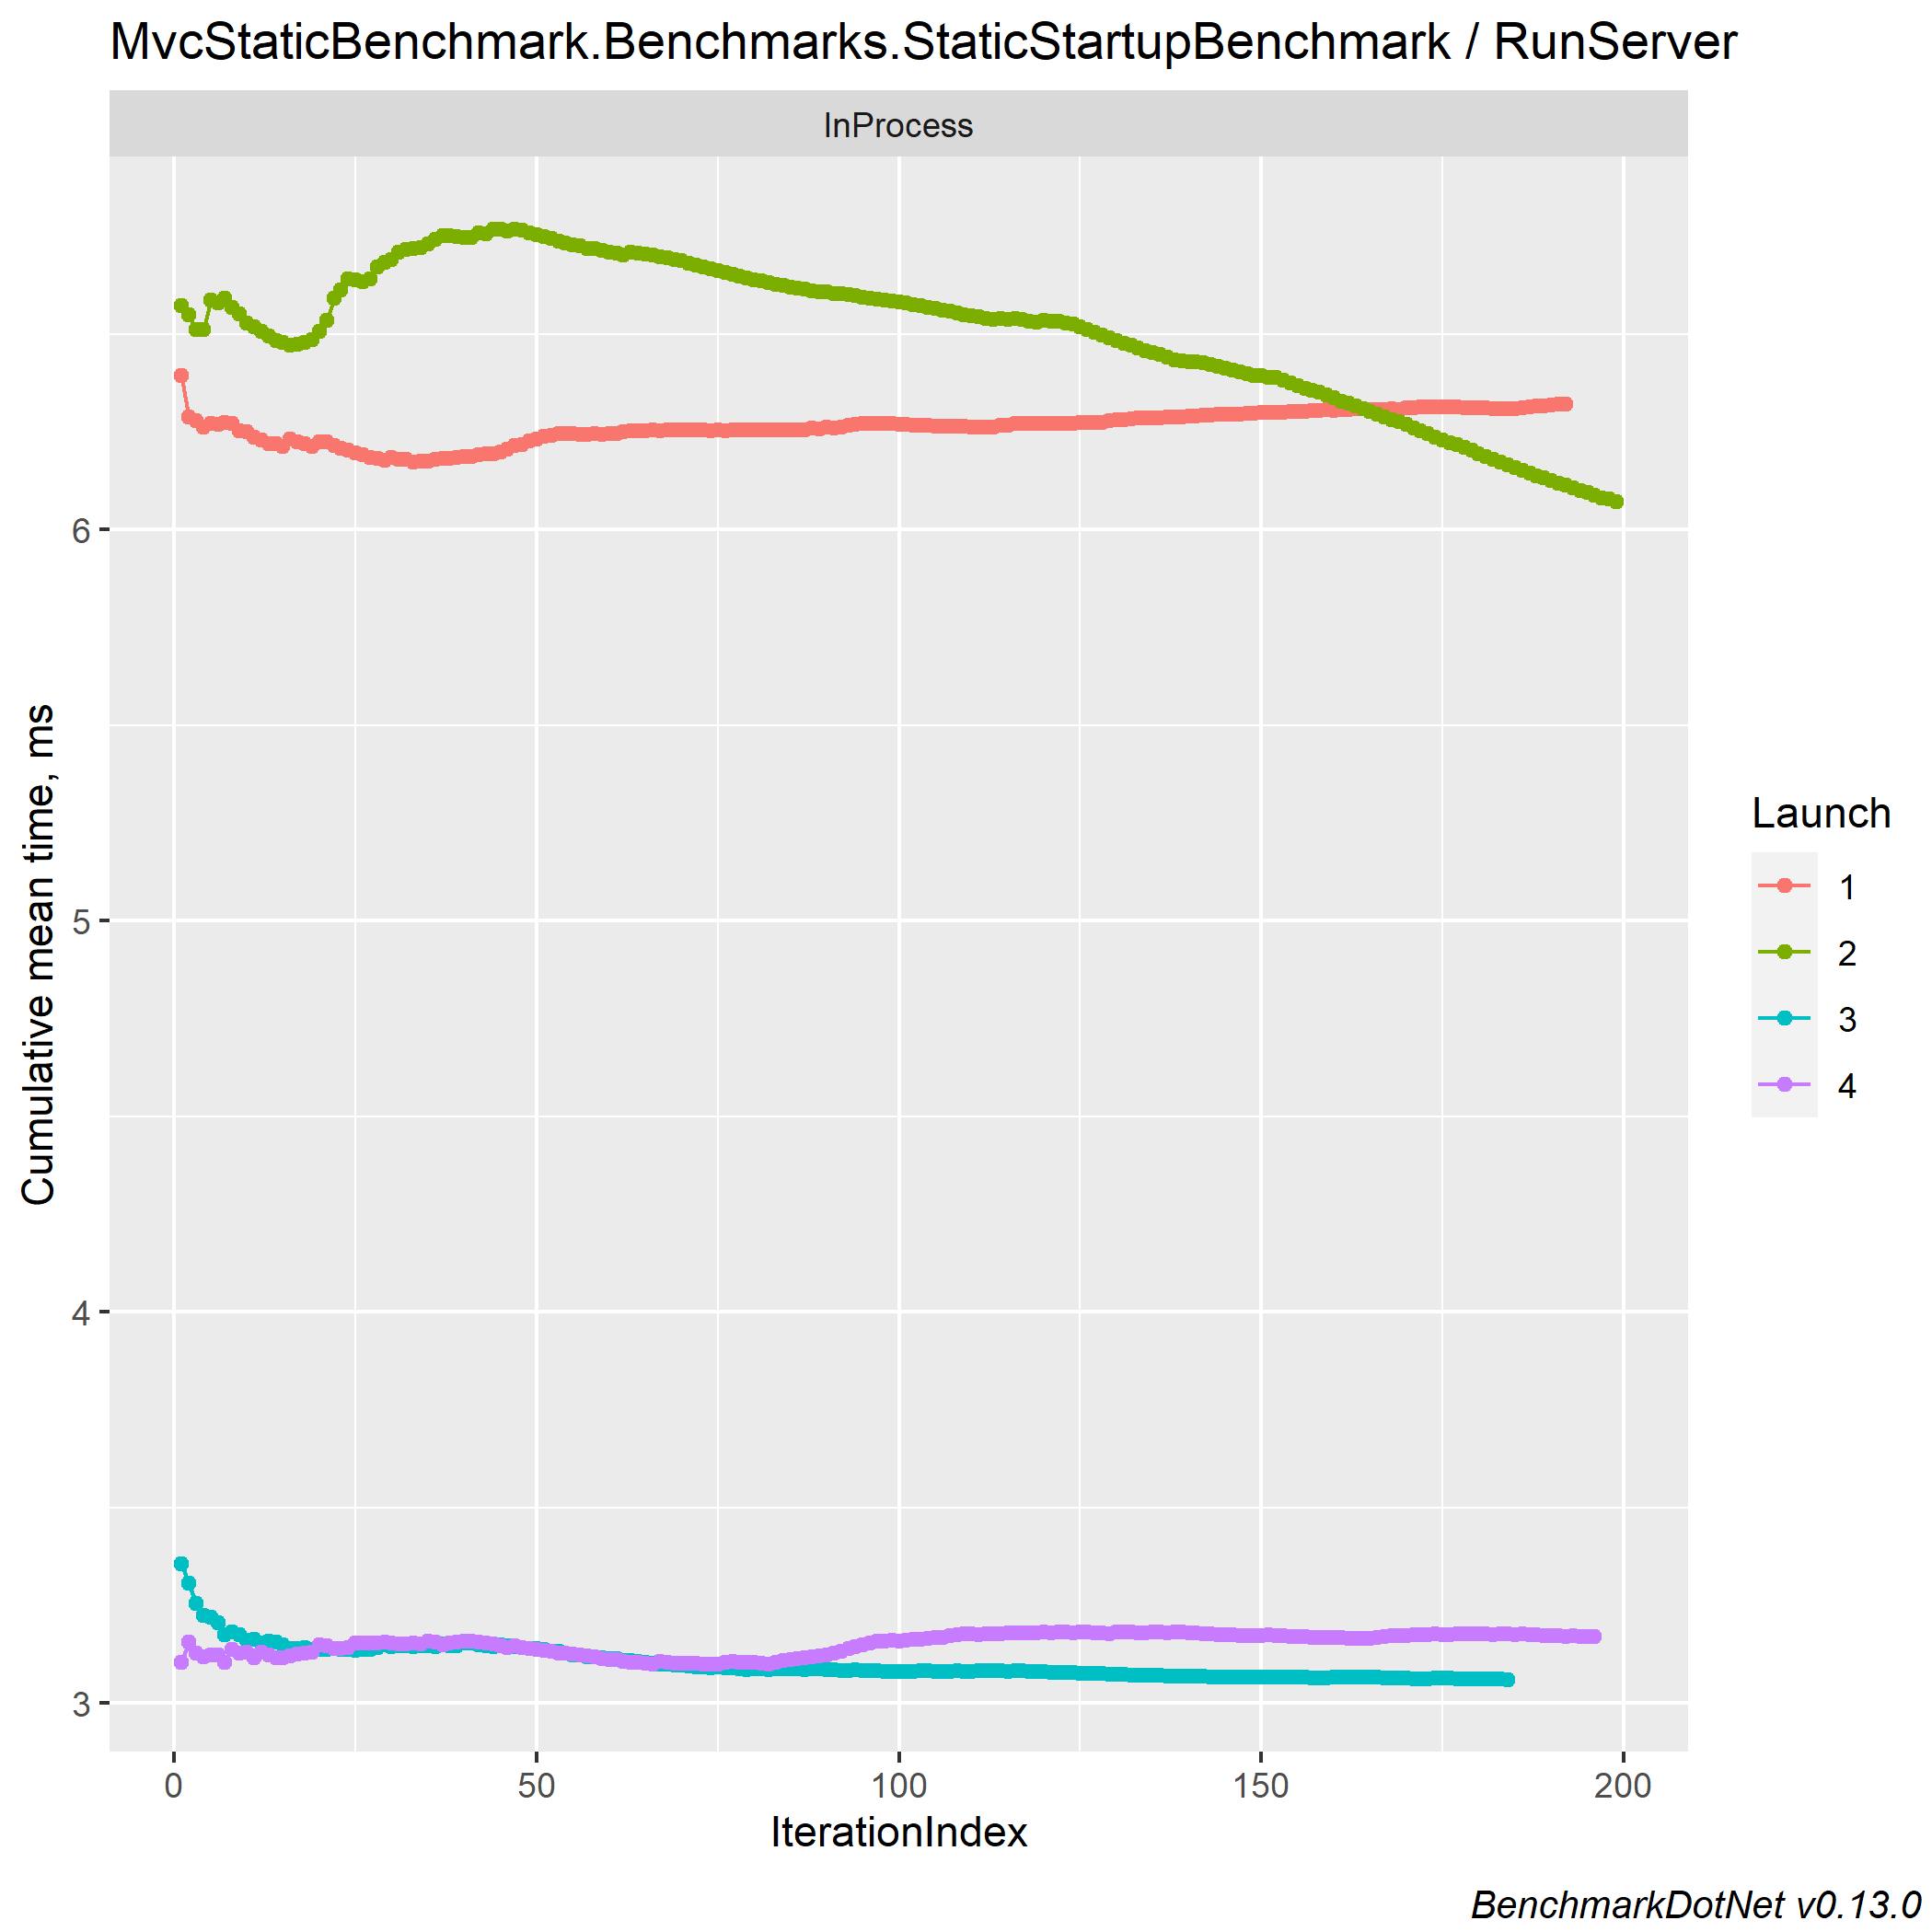
\includegraphics[width=0.8\textwidth]{graphics/MvcStaticBenchmark.Benchmarks.StaticStartupBenchmark-RunServer-cummean.png}
\caption{Average startup time of an application using static action discovery with 100 controllers}
\label{fig:static-startup-100}
\end{figure}

Expanding the application size to include 1,000 controllers, the startup time under dynamic action discovery (Figure \ref{fig:dynamic-startup-1000}) appears turbulent at the beginning of each benchmark. However, the measurements eventually stabilize around 86 milliseconds. The mean startup time for this application under dynamic action discovery is 86.02 milliseconds, with an error margin of 0.14 and a standard deviation of 1.16.

\begin{figure}[H]
\centering
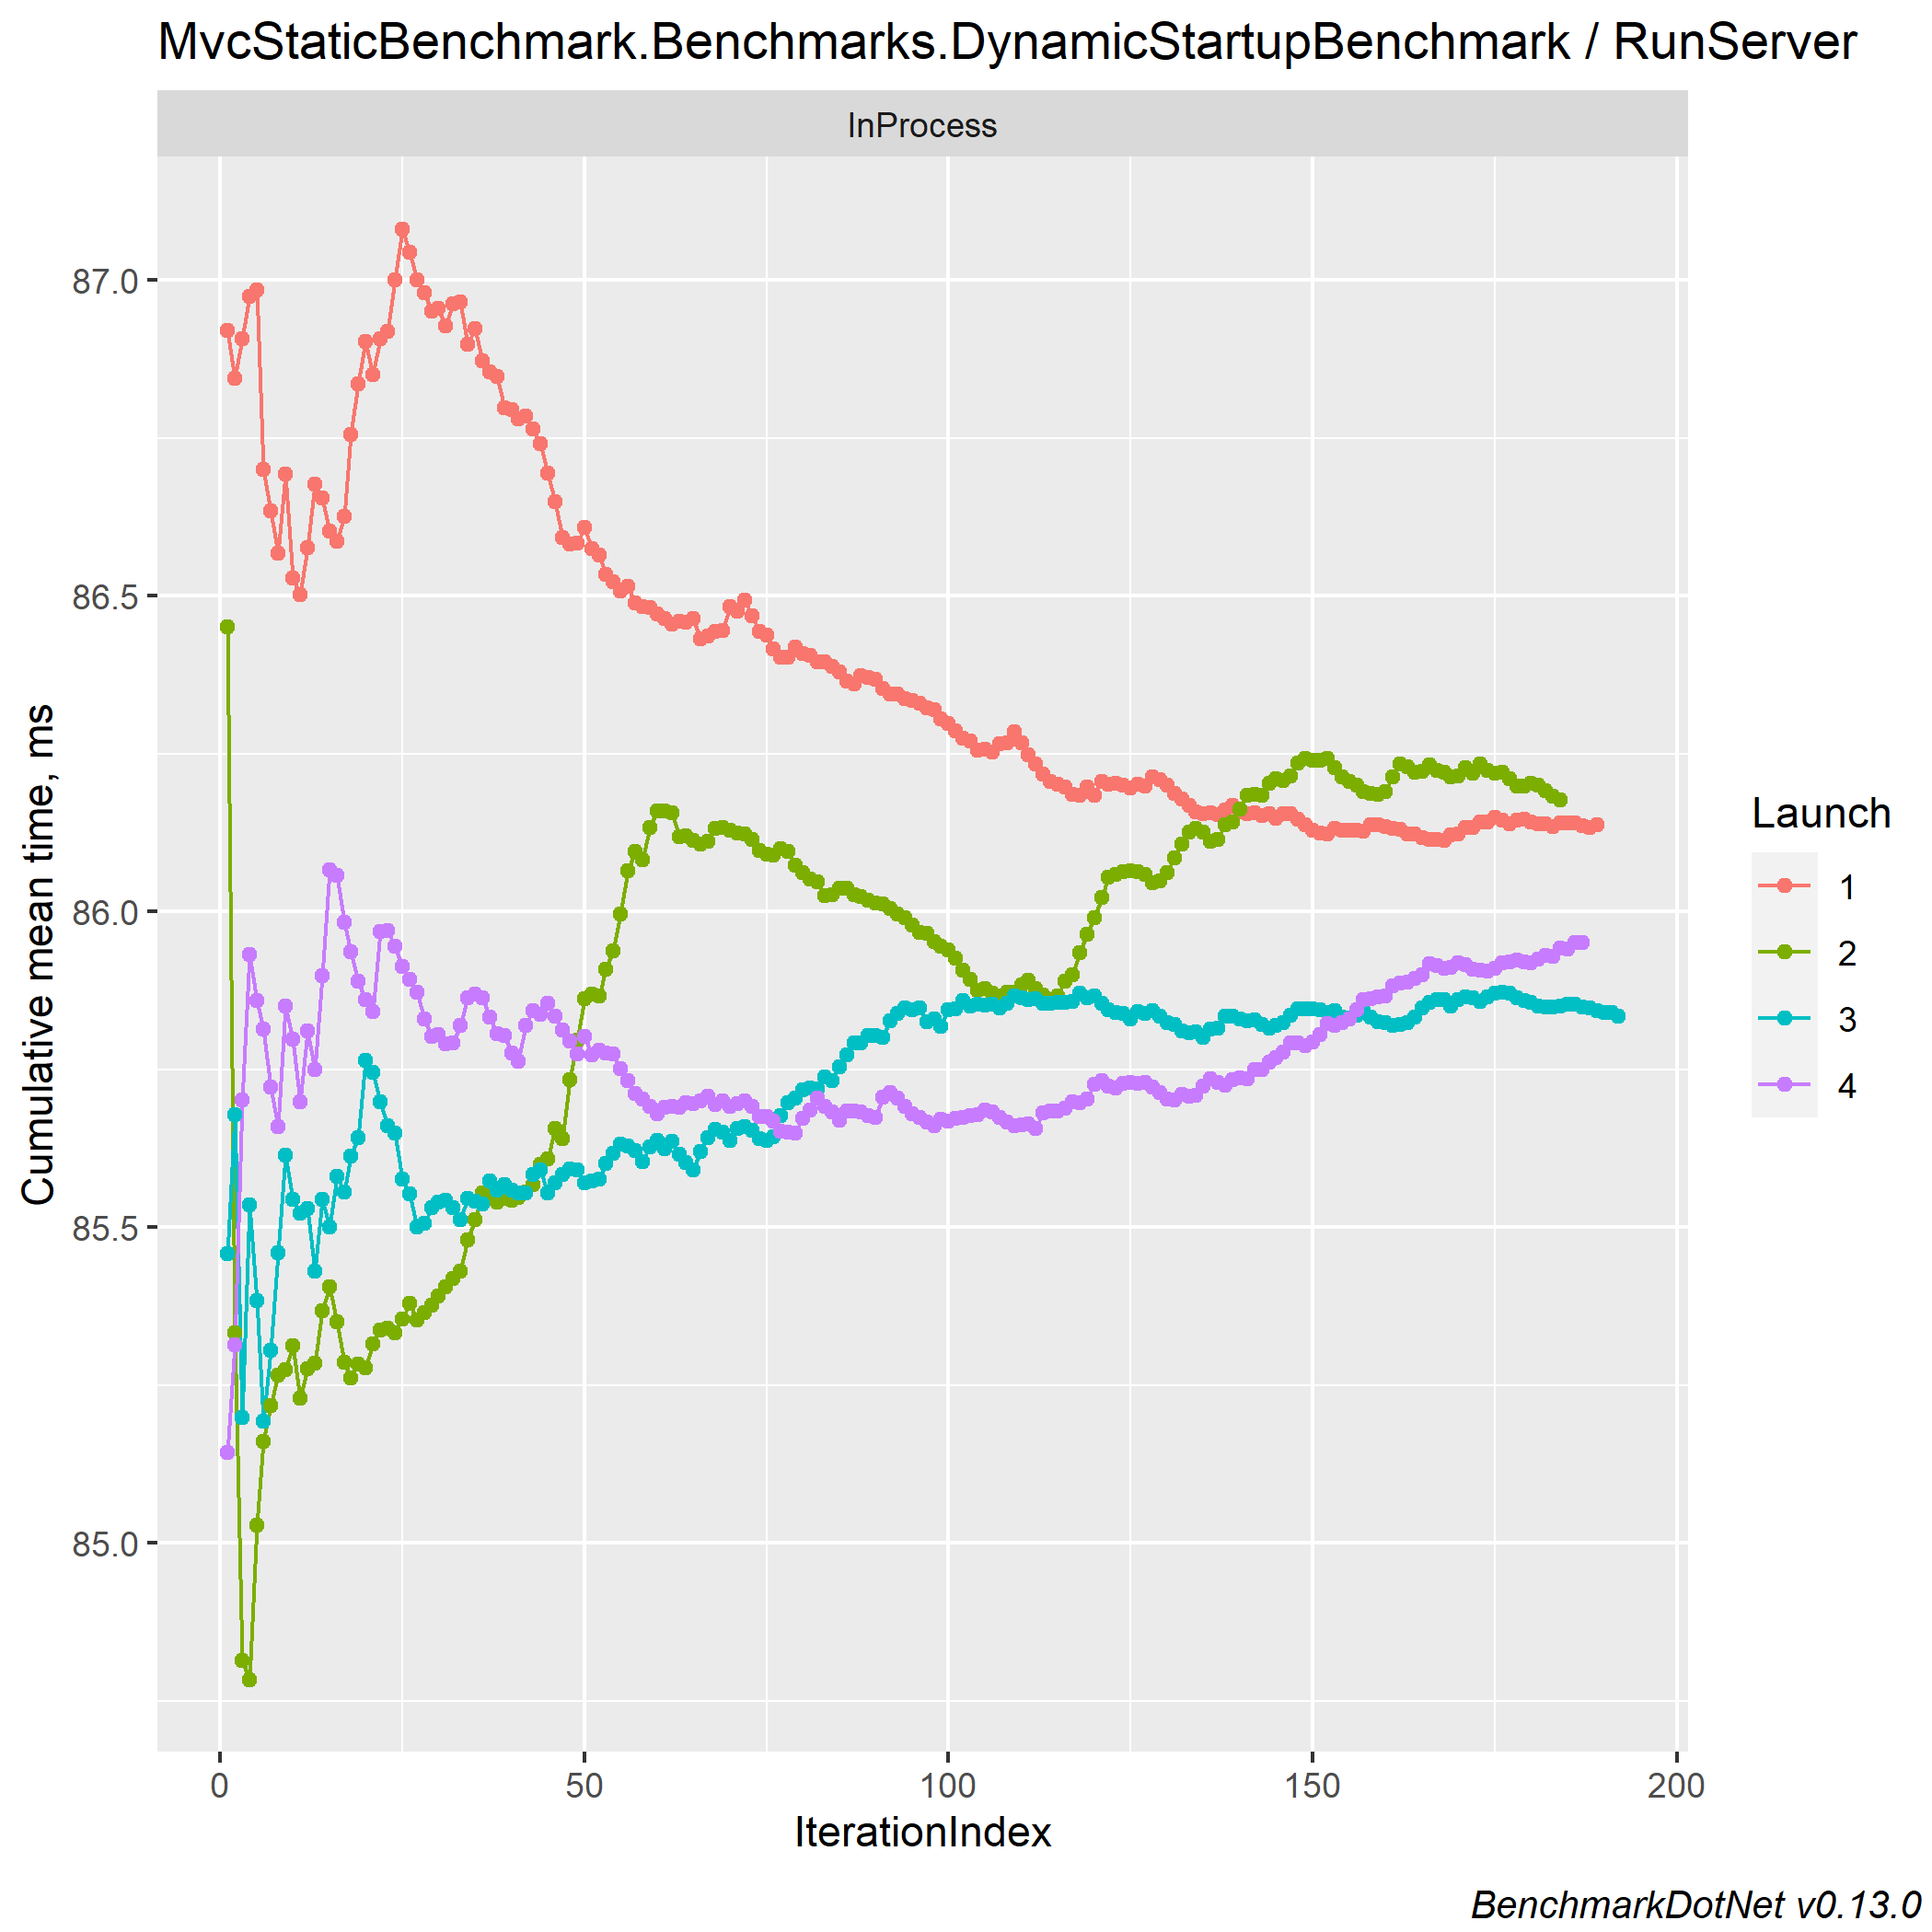
\includegraphics[width=0.8\textwidth]{graphics/MvcStaticBenchmark.Benchmarks.DynamicStartupBenchmark-RunServer-cummean 1000.png}
\caption{Average startup time of an application using dynamic action discovery with 1000 controllers}
\label{fig:dynamic-startup-1000}
\end{figure}

Figure \ref{fig:static-startup-1000} portrays the static action discovery approach for the same 1,000 controller application. Here, we observe two distinct groups of runs: the first two runs average between 16.2 and 17 milliseconds, while the latter two consistently fall between 15 and 15.7 milliseconds. The mean duration is 15.9 milliseconds, with an error of 0.084 and a standard deviation of 0.706.

\begin{figure}[H]
\centering
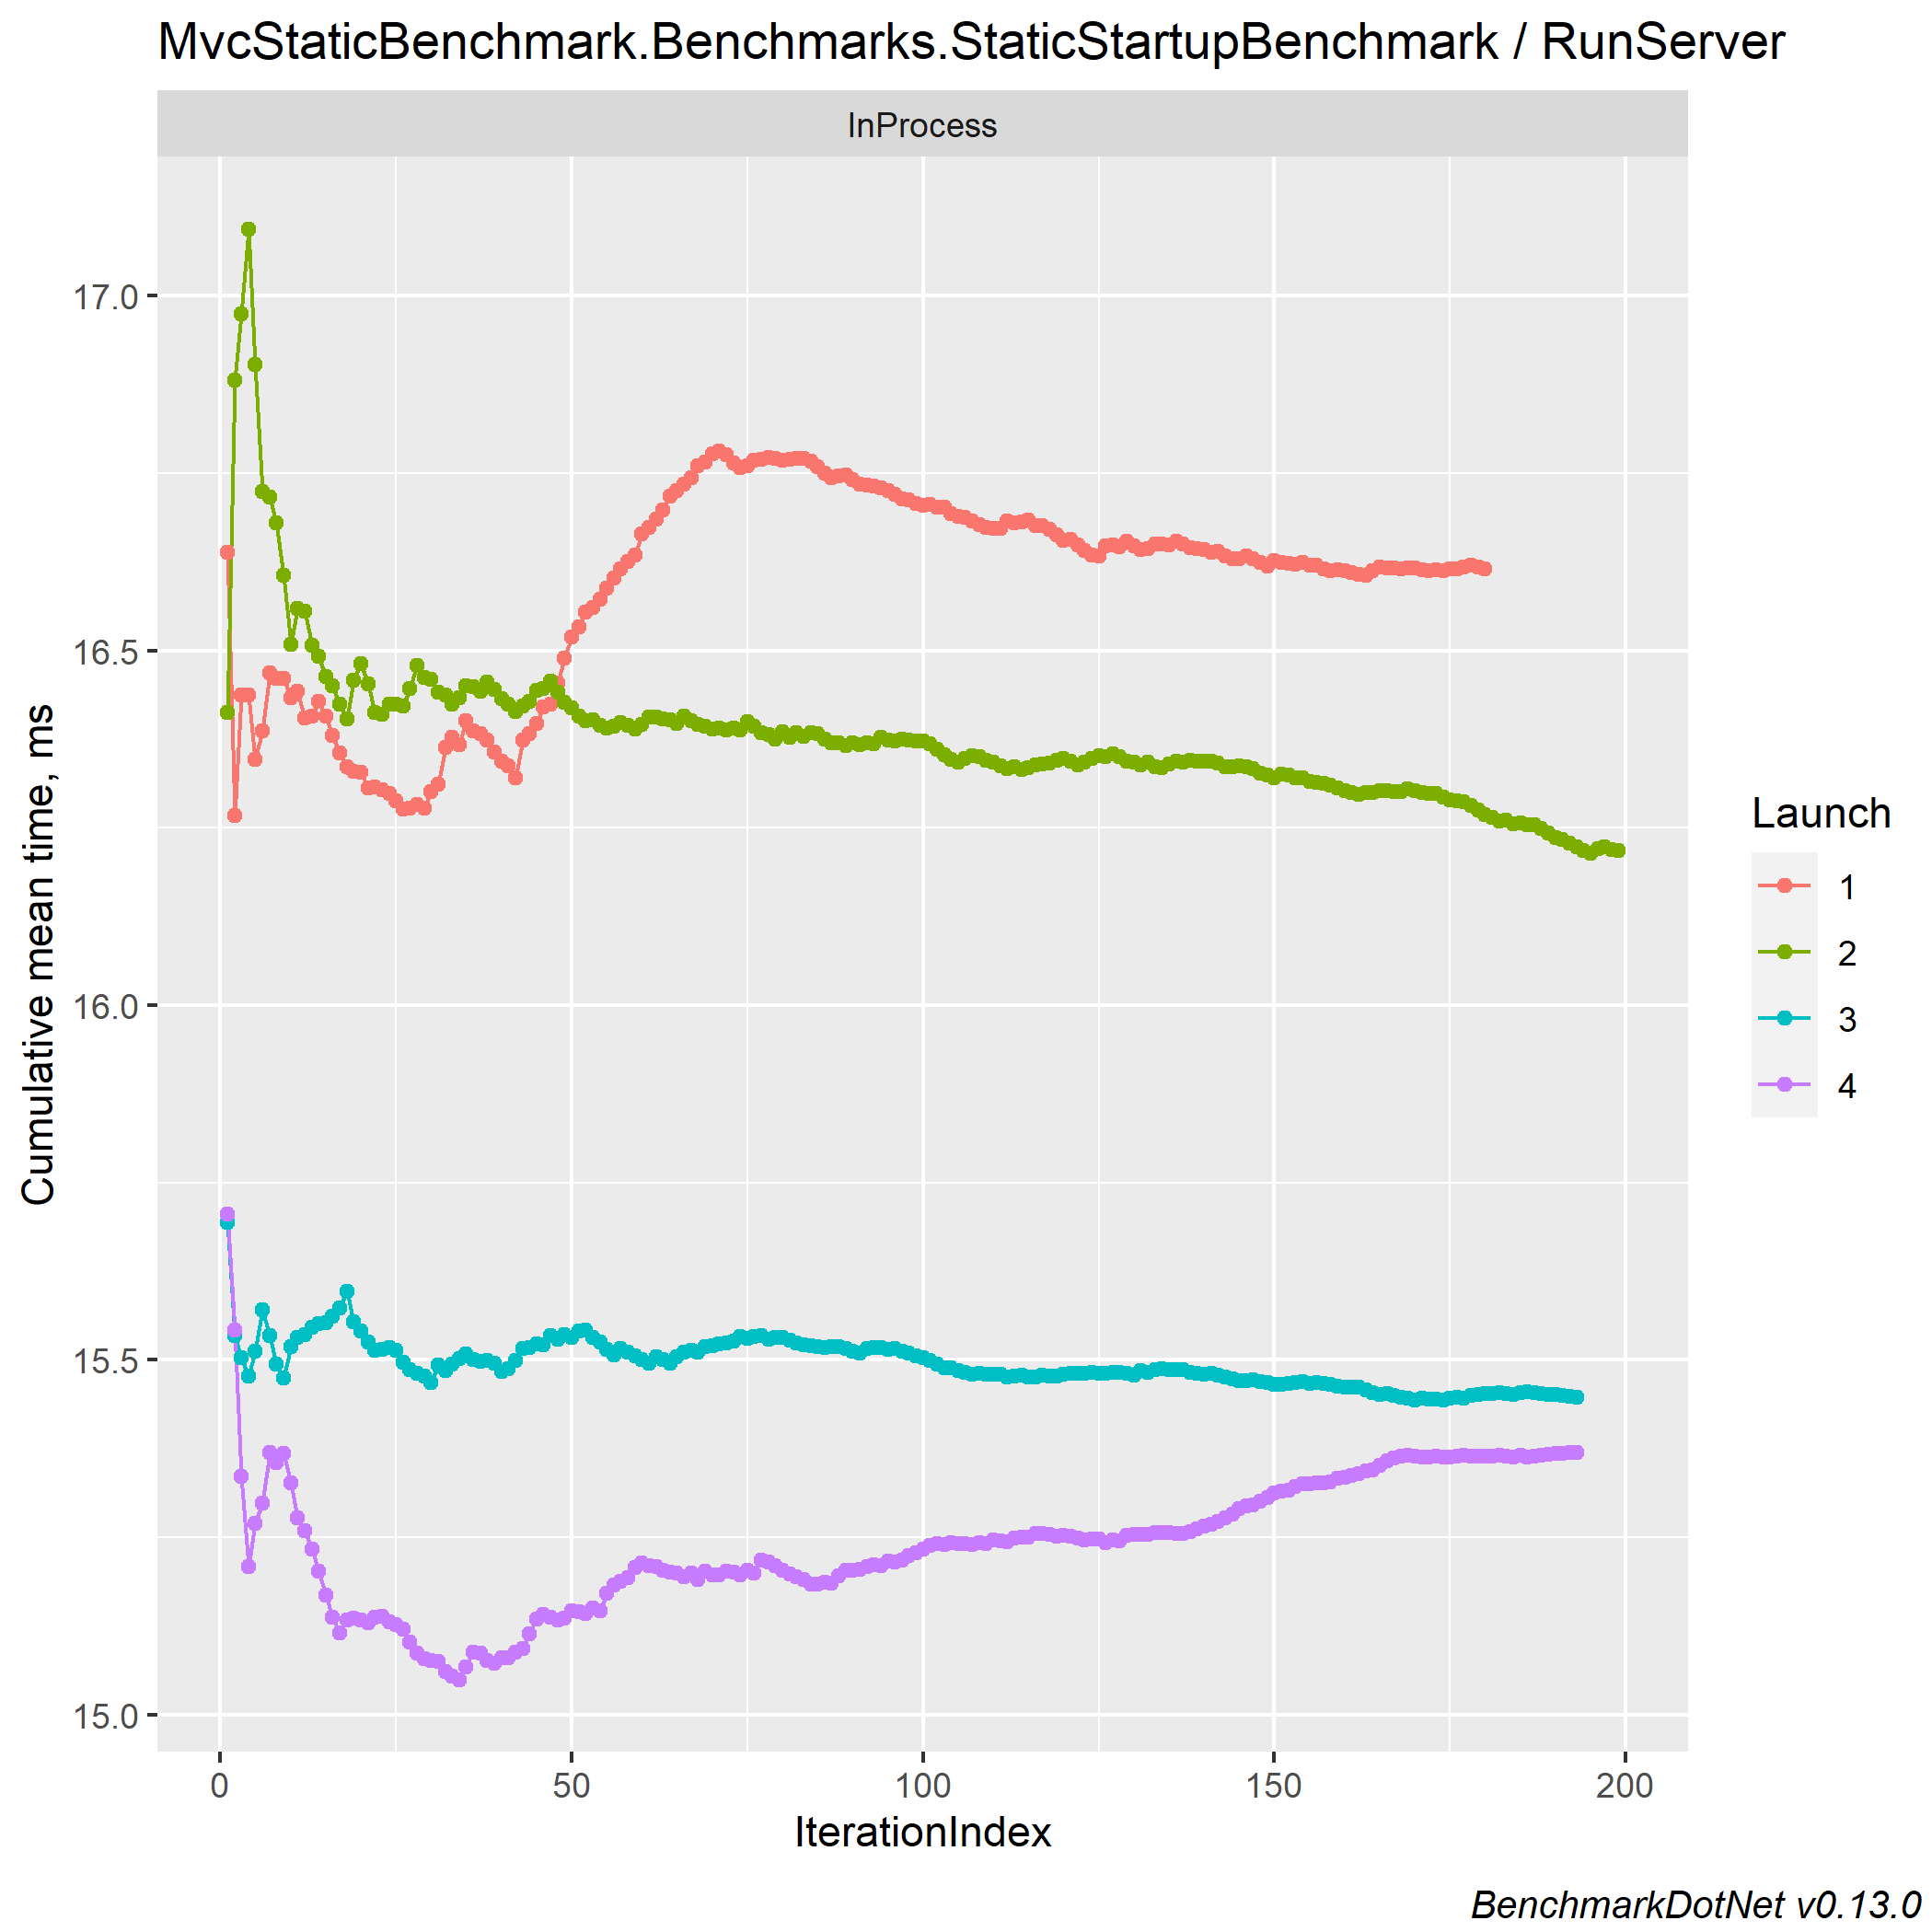
\includegraphics[width=0.8\textwidth]{graphics/MvcStaticBenchmark.Benchmarks.StaticStartupBenchmark-RunServer-cummean 1000.png}
\caption{Average startup time of an application using static action discovery with 1000 controllers}
\label{fig:static-startup-1000}
\end{figure}

Increasing the controller count to 10,000, dynamic action discovery (Figure \ref{fig:dynamic-startup-10000}) results in a fluctuation between 880 and 900 milliseconds at the outset, which ultimately stabilizes around 887 milliseconds. However, the fourth run deviates, rising to 910 milliseconds before settling to 900 milliseconds. Averaging across the four runs, the mean time is 890.6 milliseconds, with an error of 1.48 and a standard deviation of 12.41.

\begin{figure}[H]
\centering
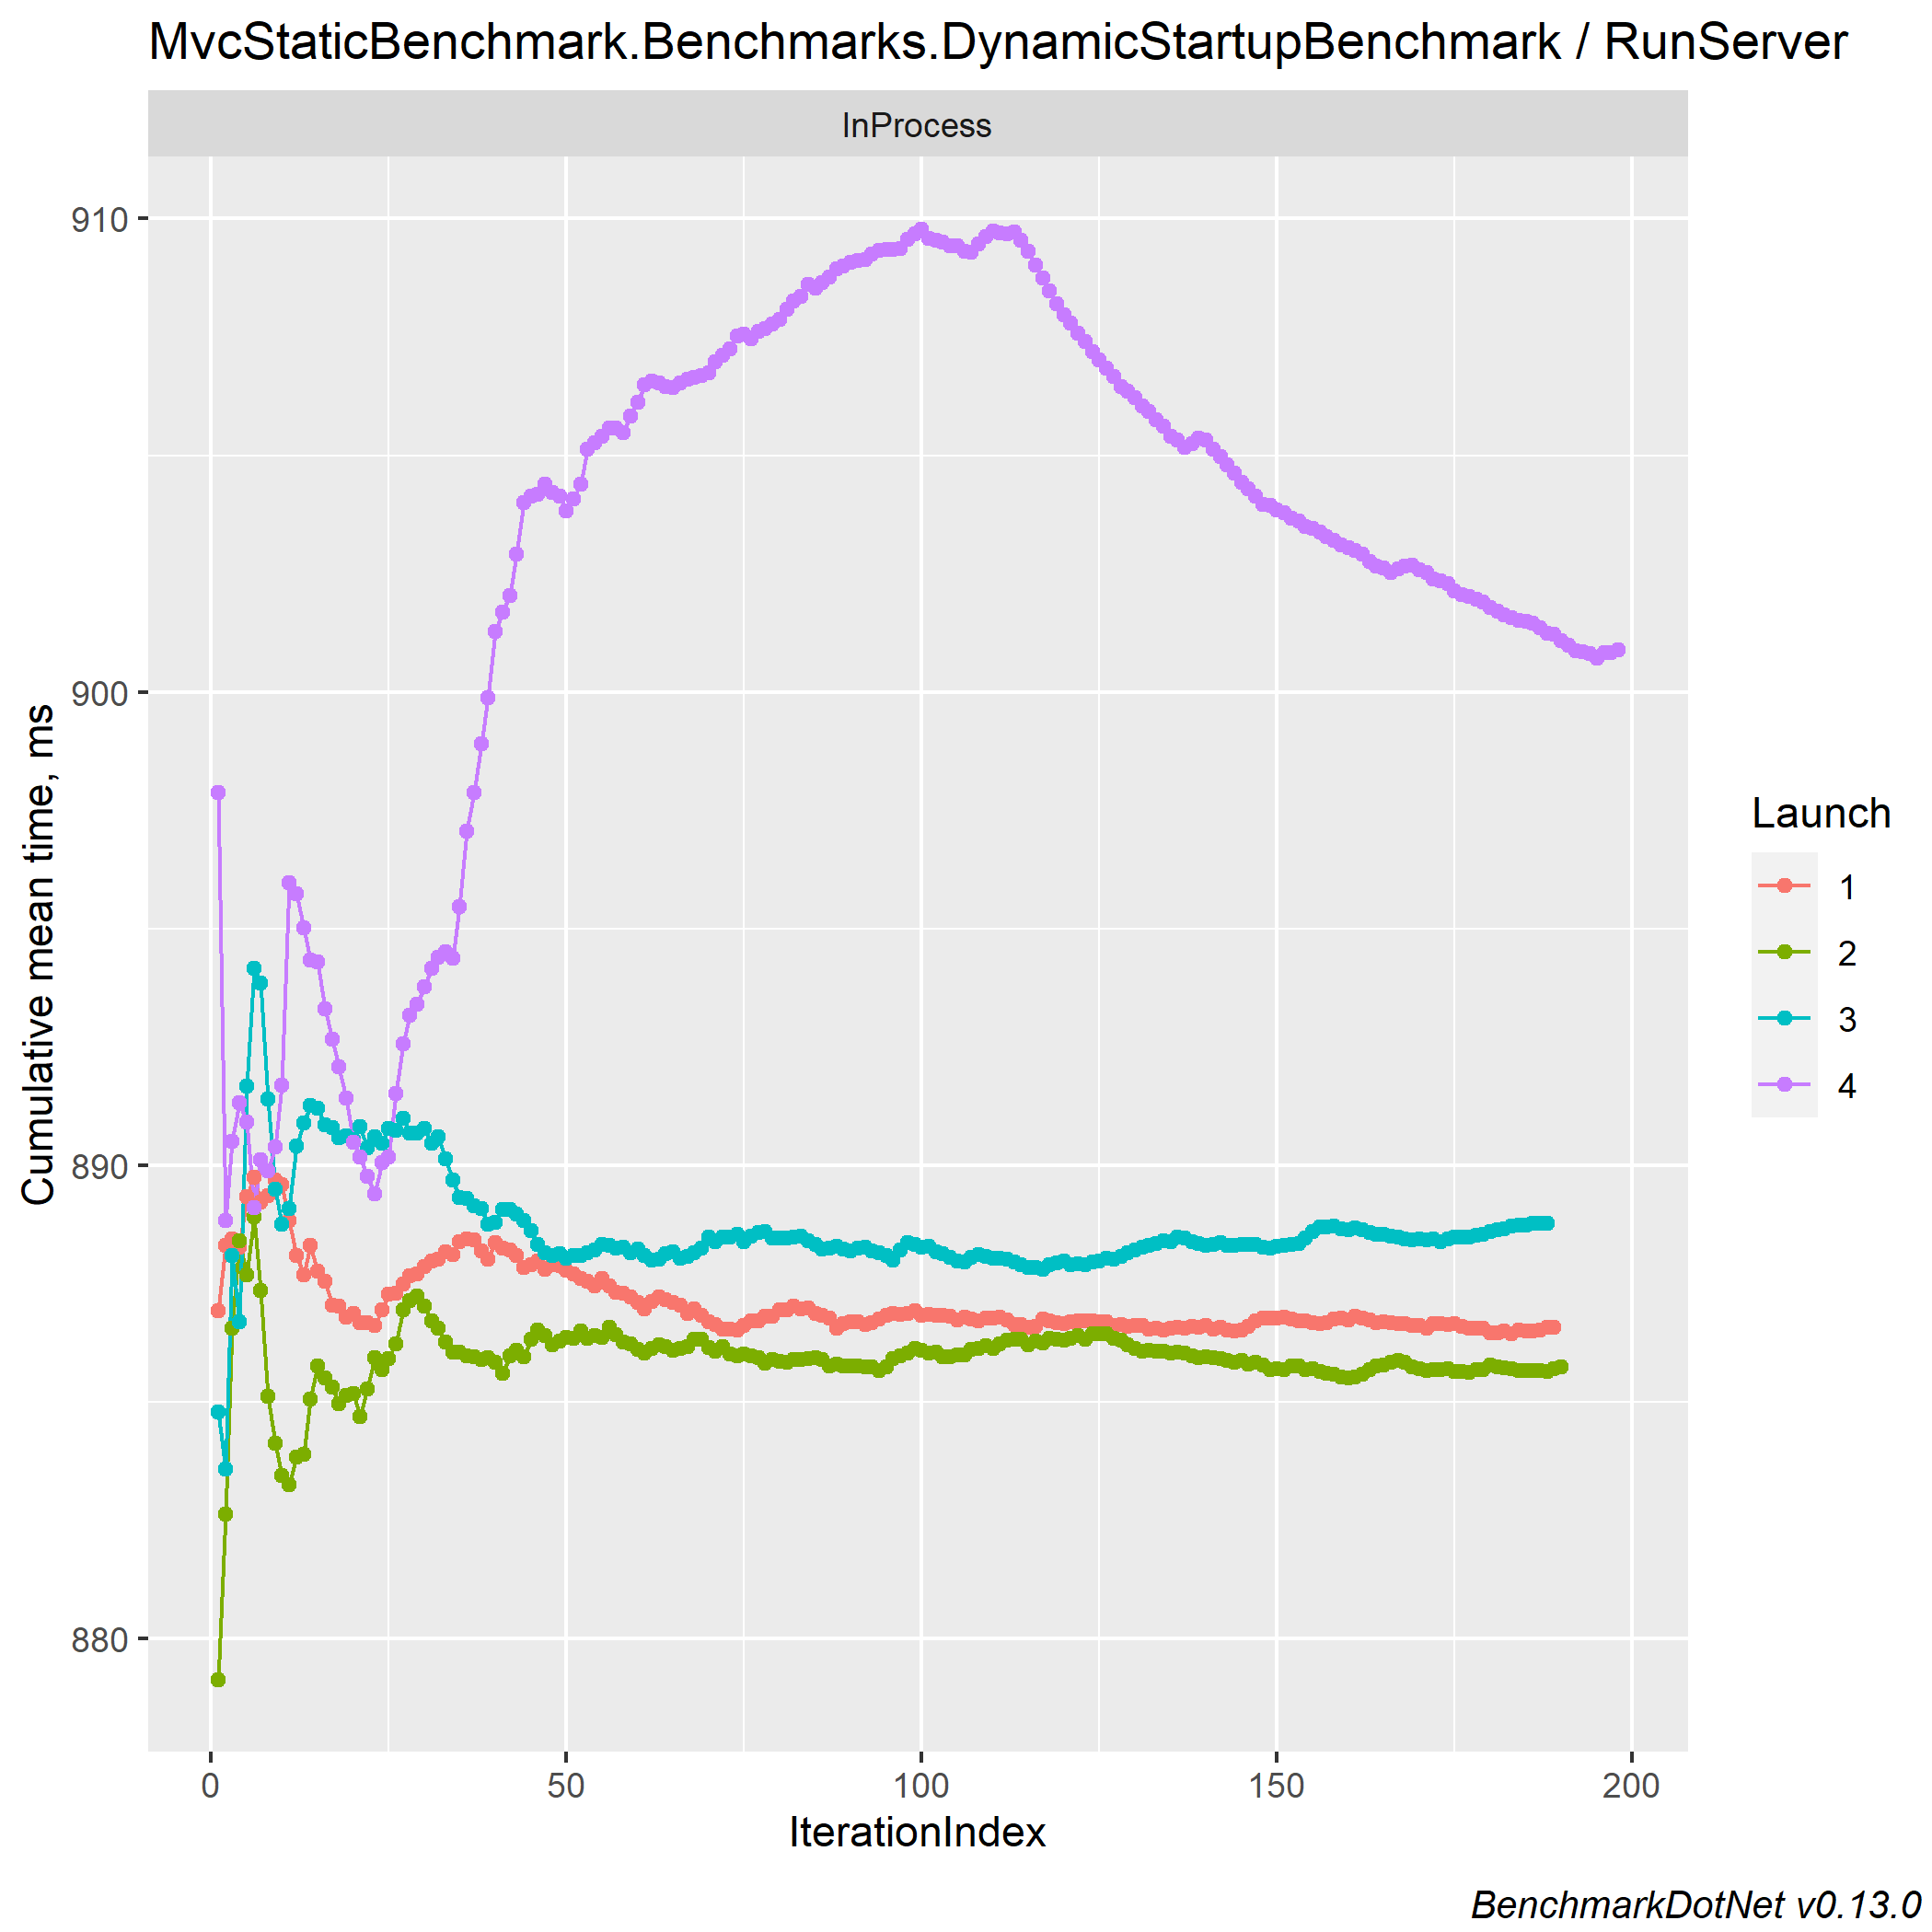
\includegraphics[width=0.8\textwidth]{graphics/MvcStaticBenchmark.Benchmarks.DynamicStartupBenchmark-RunServer-cummean 10 000.png}
\caption{Average startup time of an application using dynamic action discovery with 10,000 controllers}
\label{fig:dynamic-startup-10000}
\end{figure}

Finally, Figure \ref{fig:static-startup-10000} exhibits the startup times with static action discovery for the 10,000 controller application. The four runs initiate between 193 and 213 milliseconds, converging closer to between 197 and 207 milliseconds by the end. This benchmark presents a mean startup duration of 202 milliseconds, an error of 0.67, and a standard deviation of 5.68.

\begin{figure}[H]
\centering
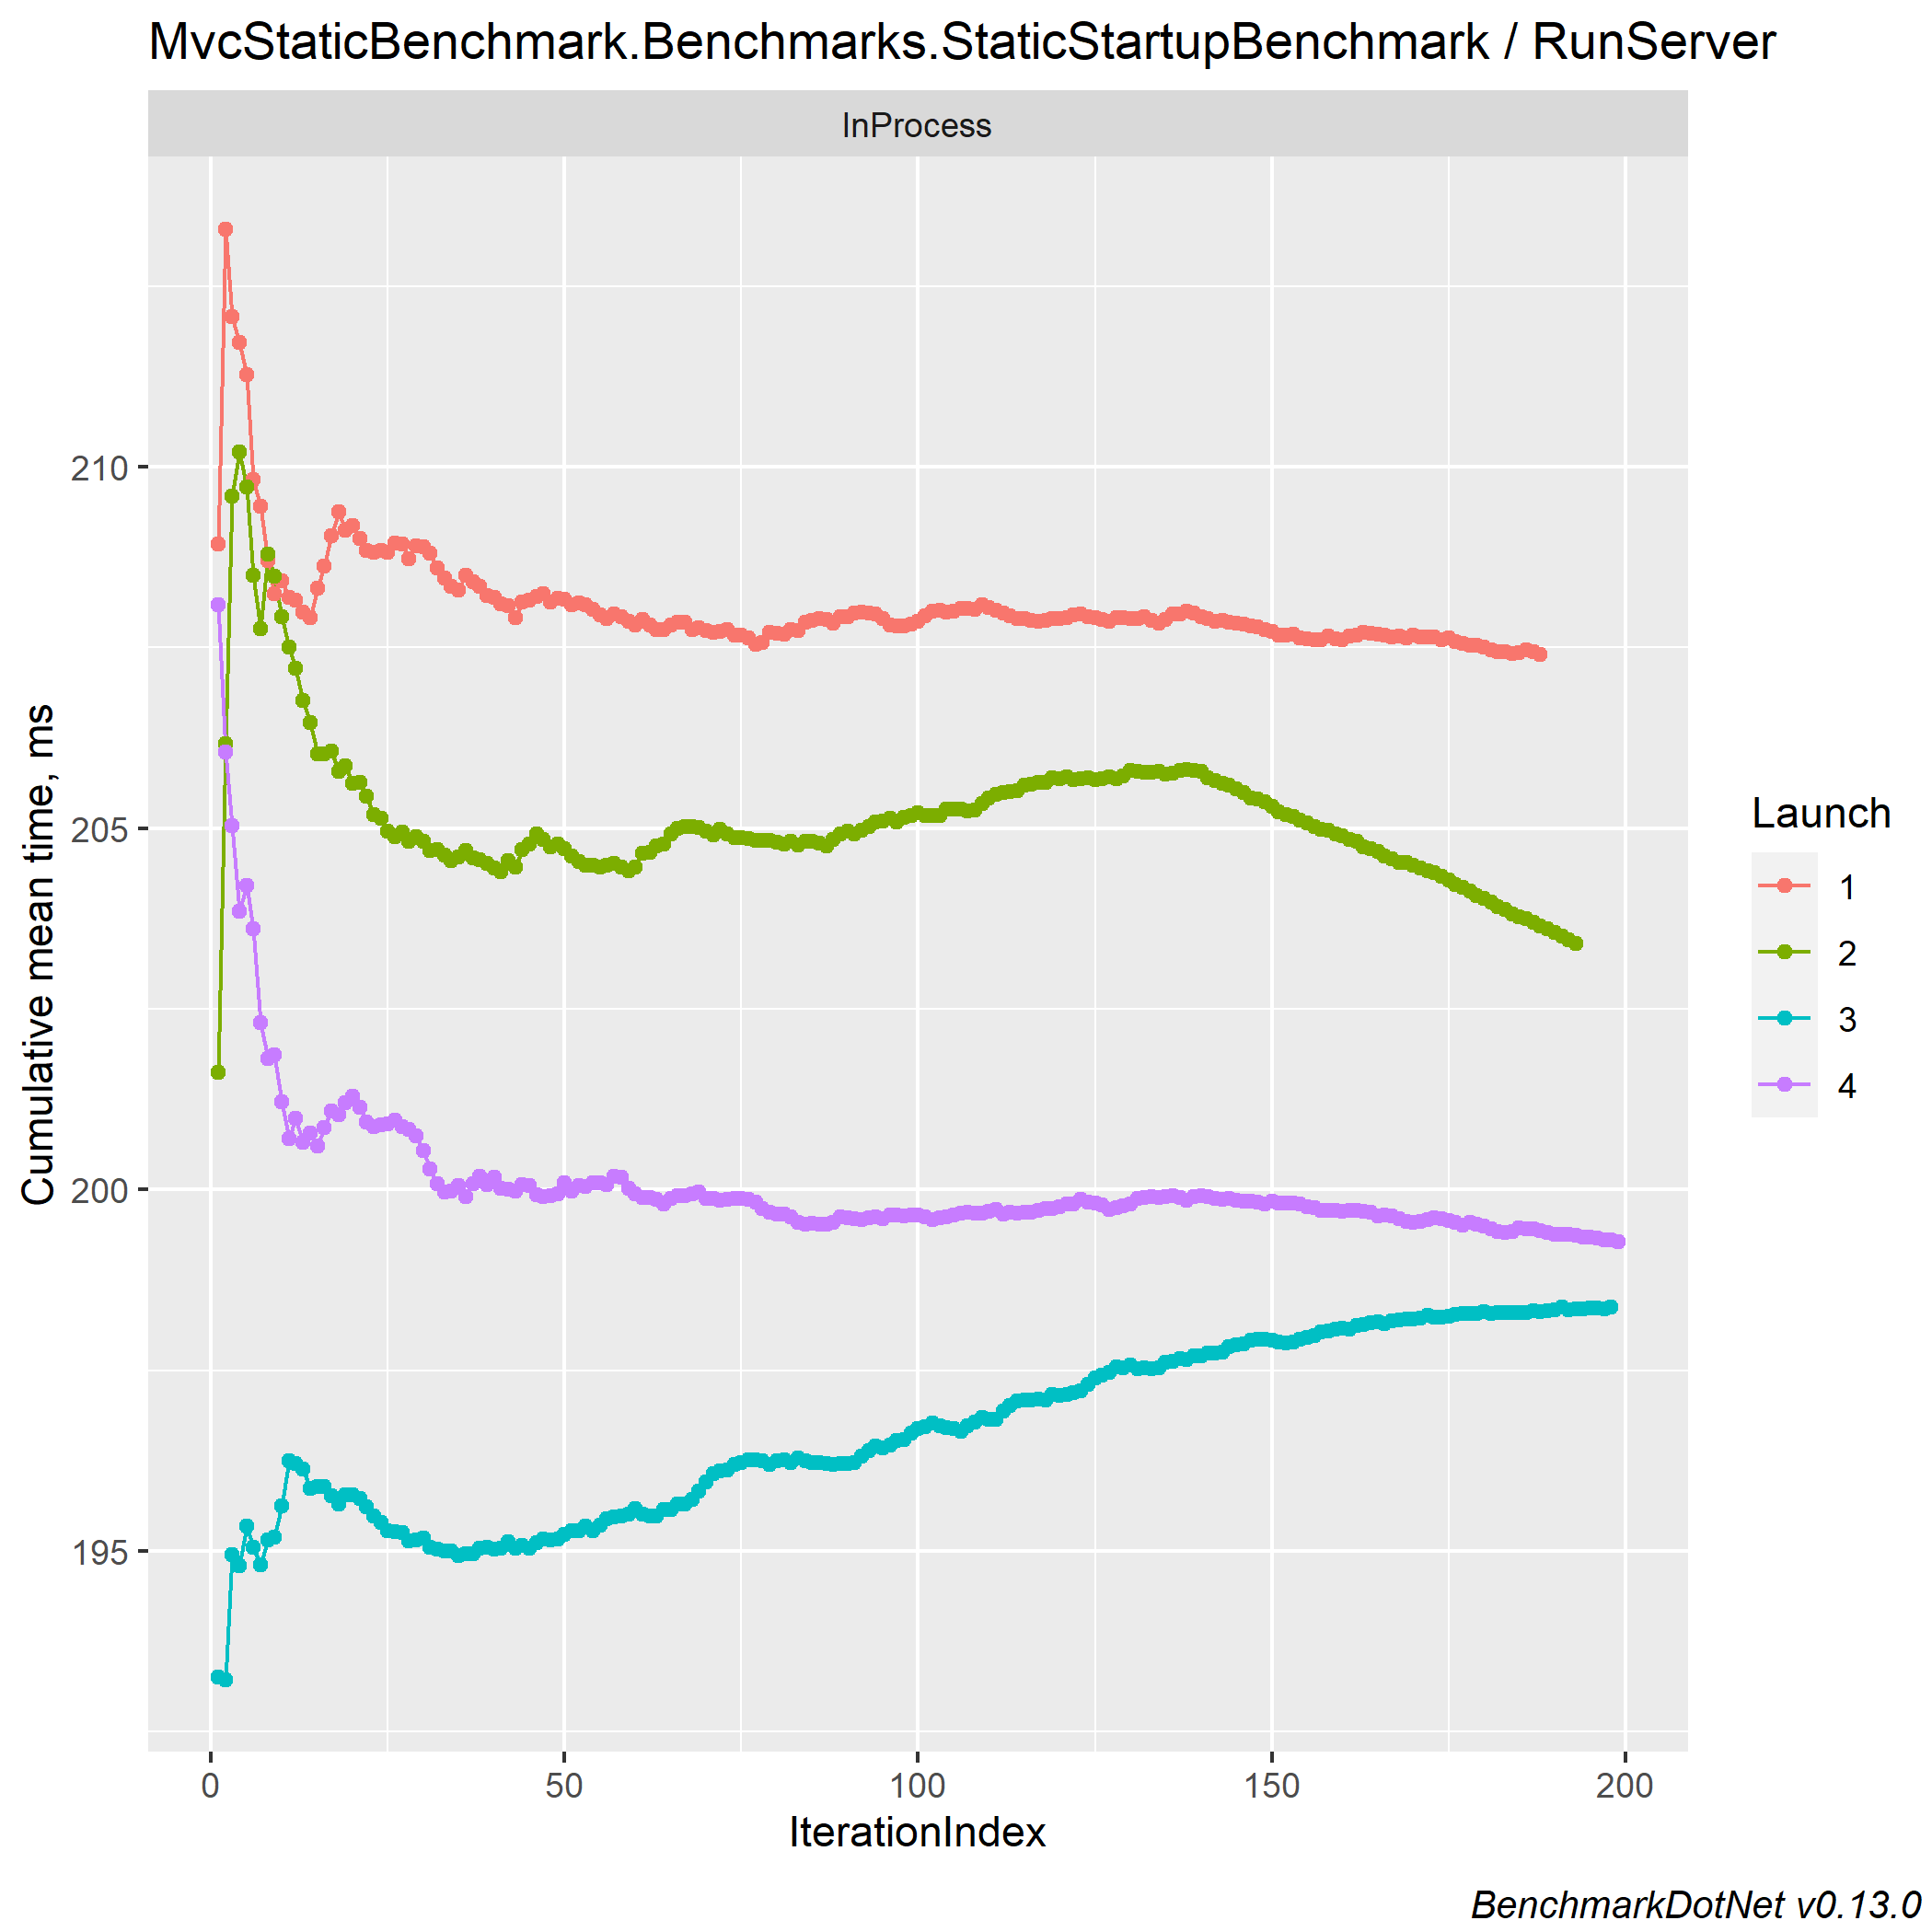
\includegraphics[width=0.8\textwidth]{graphics/MvcStaticBenchmark.Benchmarks.StaticStartupBenchmark-RunServer-cummean 10 000.png}
\caption{Average startup time of an application using static action discovery with 10,000 controllers}
\label{fig:static-startup-10000}
\end{figure}

Furthermore, Figure \ref{fig:startup-time-results} visualizes the mean startup time as a bar chart, with groups representing applications of 100, 1,000, or 10,000 controllers. Each group comprises the mean startup times of both static (right) and dynamic (left) action discoveries. This visualization simplifies comparisons between the methods across varying application sizes.

\begin{figure}[H]
\centering
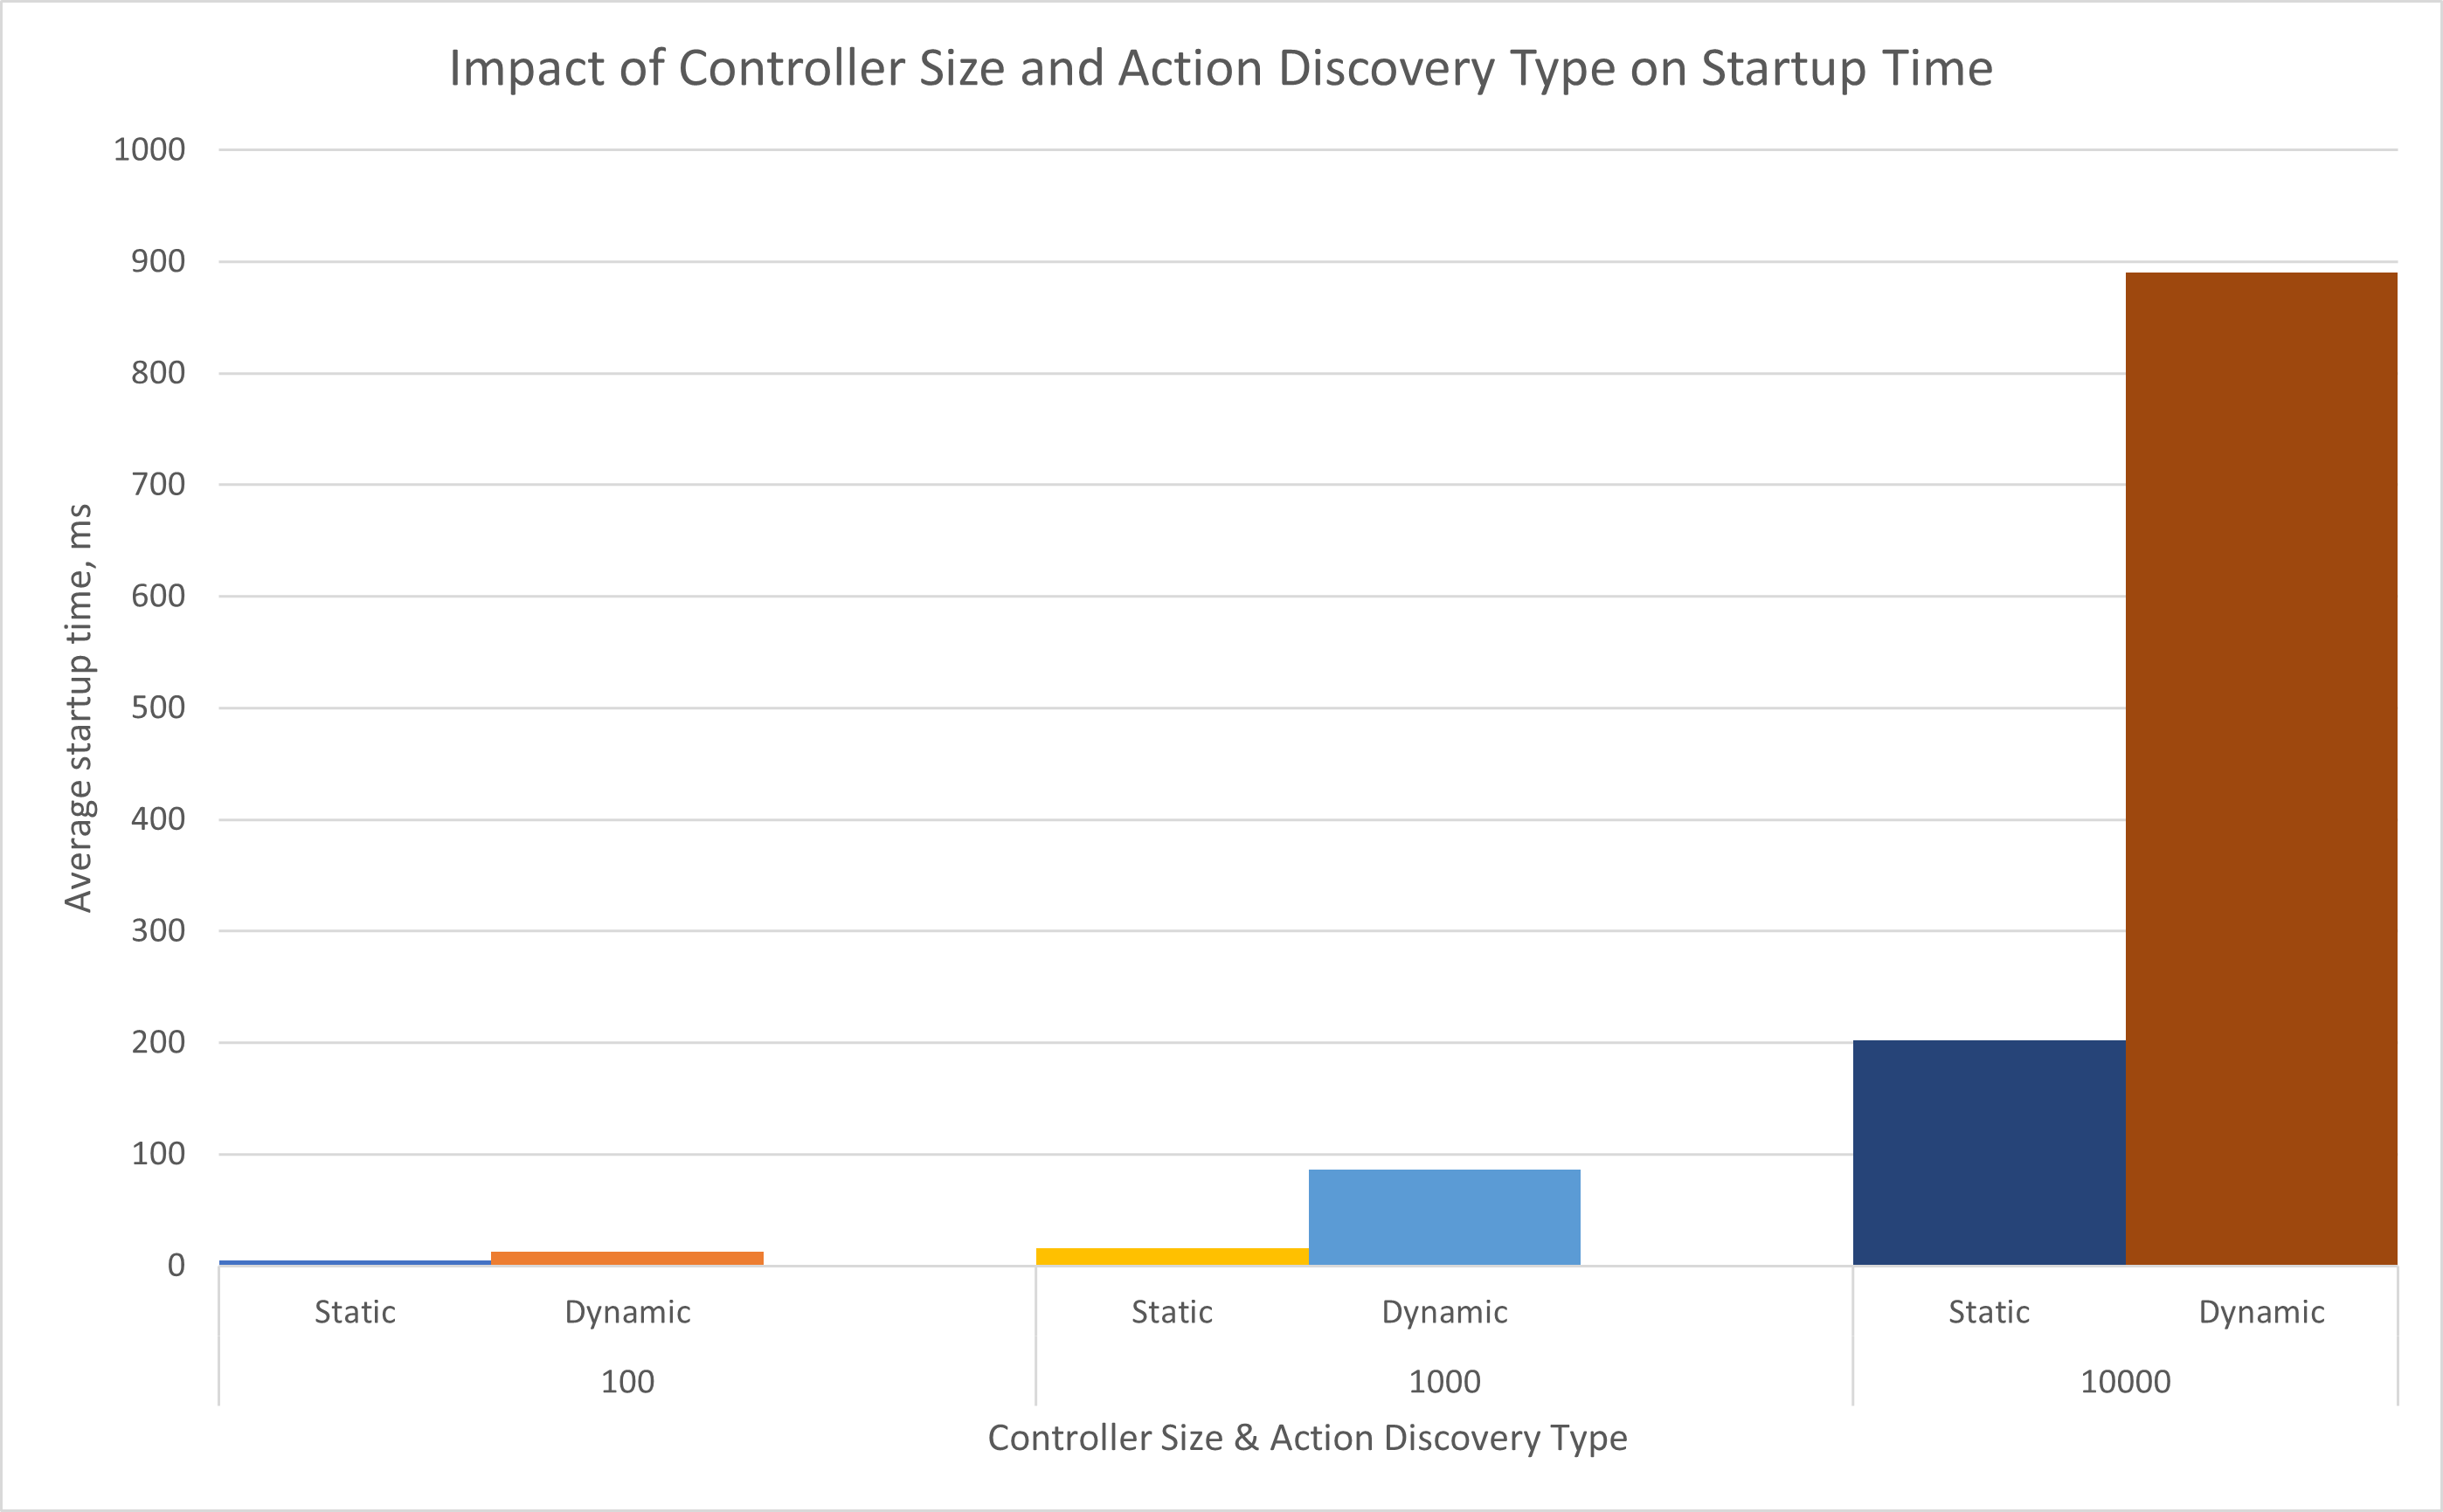
\includegraphics[width=0.8\textwidth]{graphics/Impact of Controller Size and Action Discovery Type on Startup Time.png}
\caption{Impact of Controller Size and Action Discovery Type on Startup Time}
\label{fig:startup-time-results}
\end{figure}

\section{Build Duration}

For an application with 100 controllers utilizing static action discovery, the mean build time was recorded as 1888 milliseconds. Across the 100 measurements, this mean time demonstrated an error of 135 and a standard deviation of 398. By comparison, the same application using dynamic action discovery averaged a shorter build time of 1566 milliseconds, with an error of 24 and a standard deviation of 71.

Escalating to an application size of 1,000 controllers, the mean build time for the static action discovery variant was 4162 milliseconds. This result was associated with an error of 102 and a standard deviation of 302. On the other hand, the dynamic action discovery method posted an average build time of 1779 milliseconds, with an error of 28 and a standard deviation of 81.

Finally, the largest application with 10,000 controllers was analyzed. Here, the static action discovery approach resulted in an average build time of 47276 milliseconds, accompanied by an error of 881 and a standard deviation of 2599. In contrast, employing dynamic action discovery resulted in a lower mean build time of 5843 milliseconds, along with an error of 66 and a standard deviation of 196.

Figure \ref{fig:build-time-results} visually represents these results as a bar chart, categorized by the number of controllers in each application. Within each group, the static action discovery value is displayed on the right, while the dynamic action discovery value is presented on the left. This arrangement allows for an intuitive comparison of build times between the two methods across applications of varying sizes.

\begin{figure}[H]
\centering
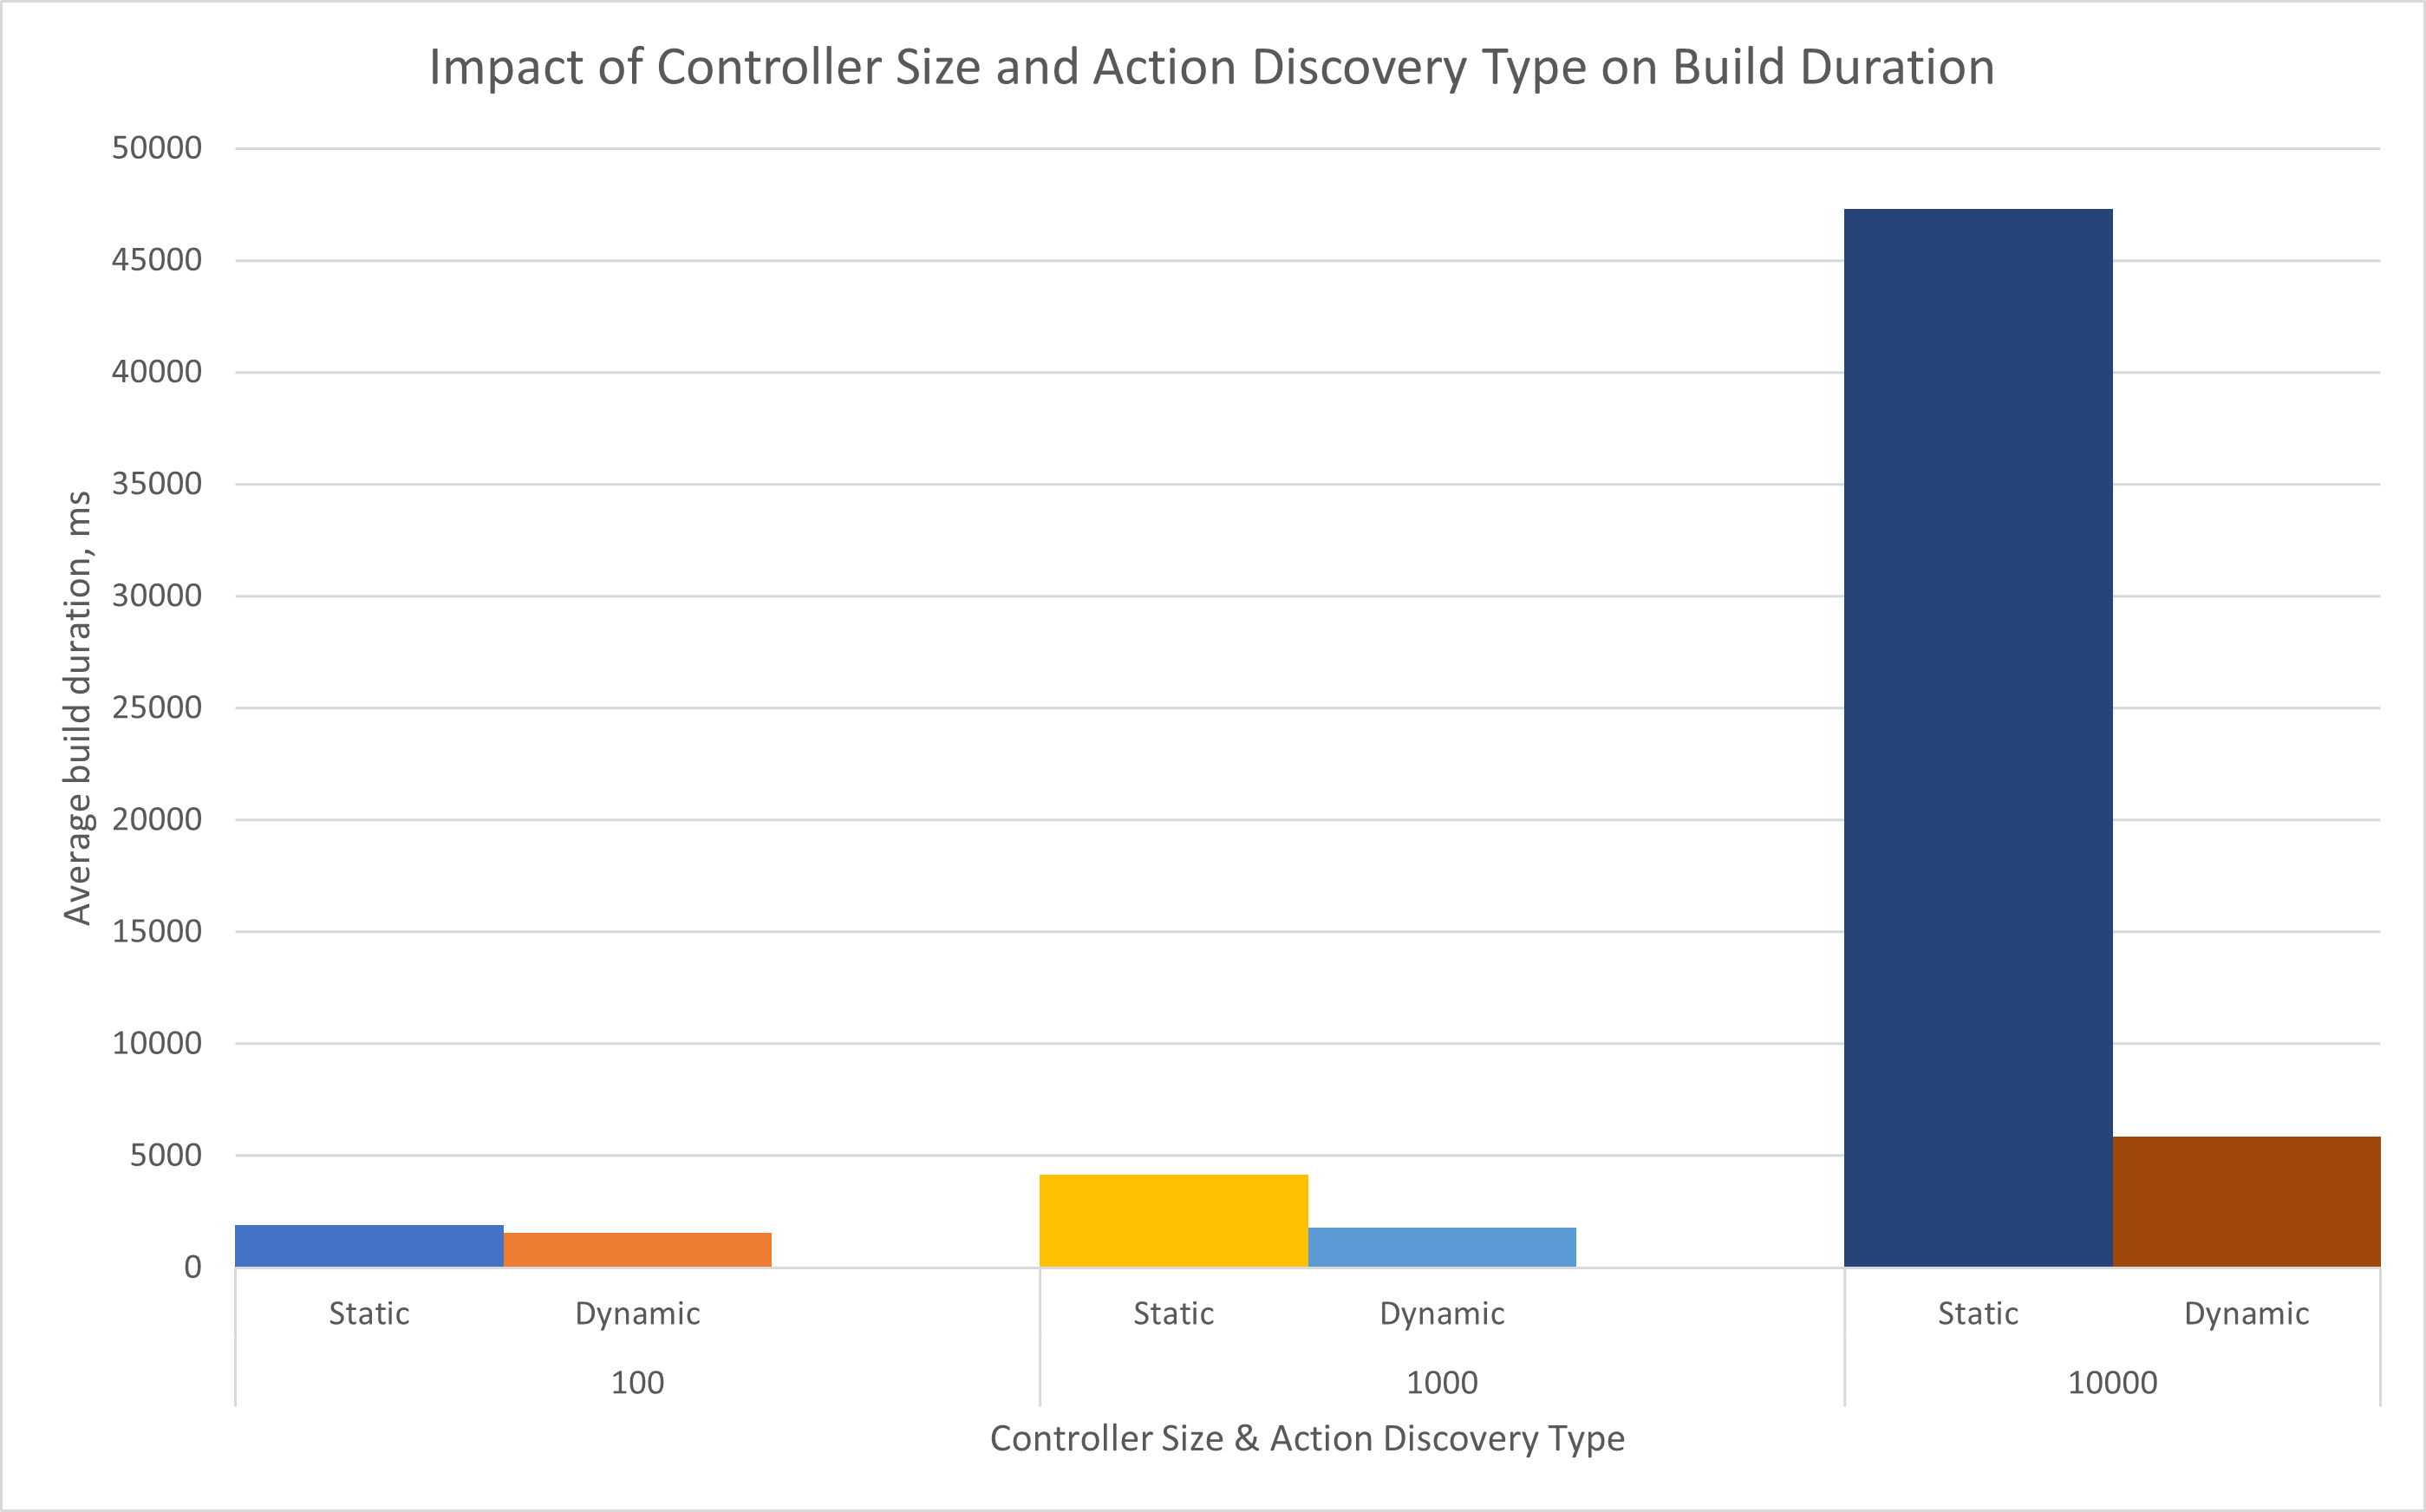
\includegraphics[width=0.8\textwidth]{graphics/Impact of Controller Size and Action Discovery Type on Build Duration.png}
\caption{Impact of Controller Size and Action Discovery Type on Build Duration}
\label{fig:build-time-results}
\end{figure}

\section{Memory Usage during Startup}

Unlike the other metrics, memory usage measurements do not have an error or standard deviation, as the execution is deterministic, and the values remain consistent throughout each measurement.

The following Figure \ref{fig:memory-usage-results} provides a comprehensive overview of memory usage across each application, differentiated by the static and dynamic action discovery methods.

\begin{figure}[H]
\centering
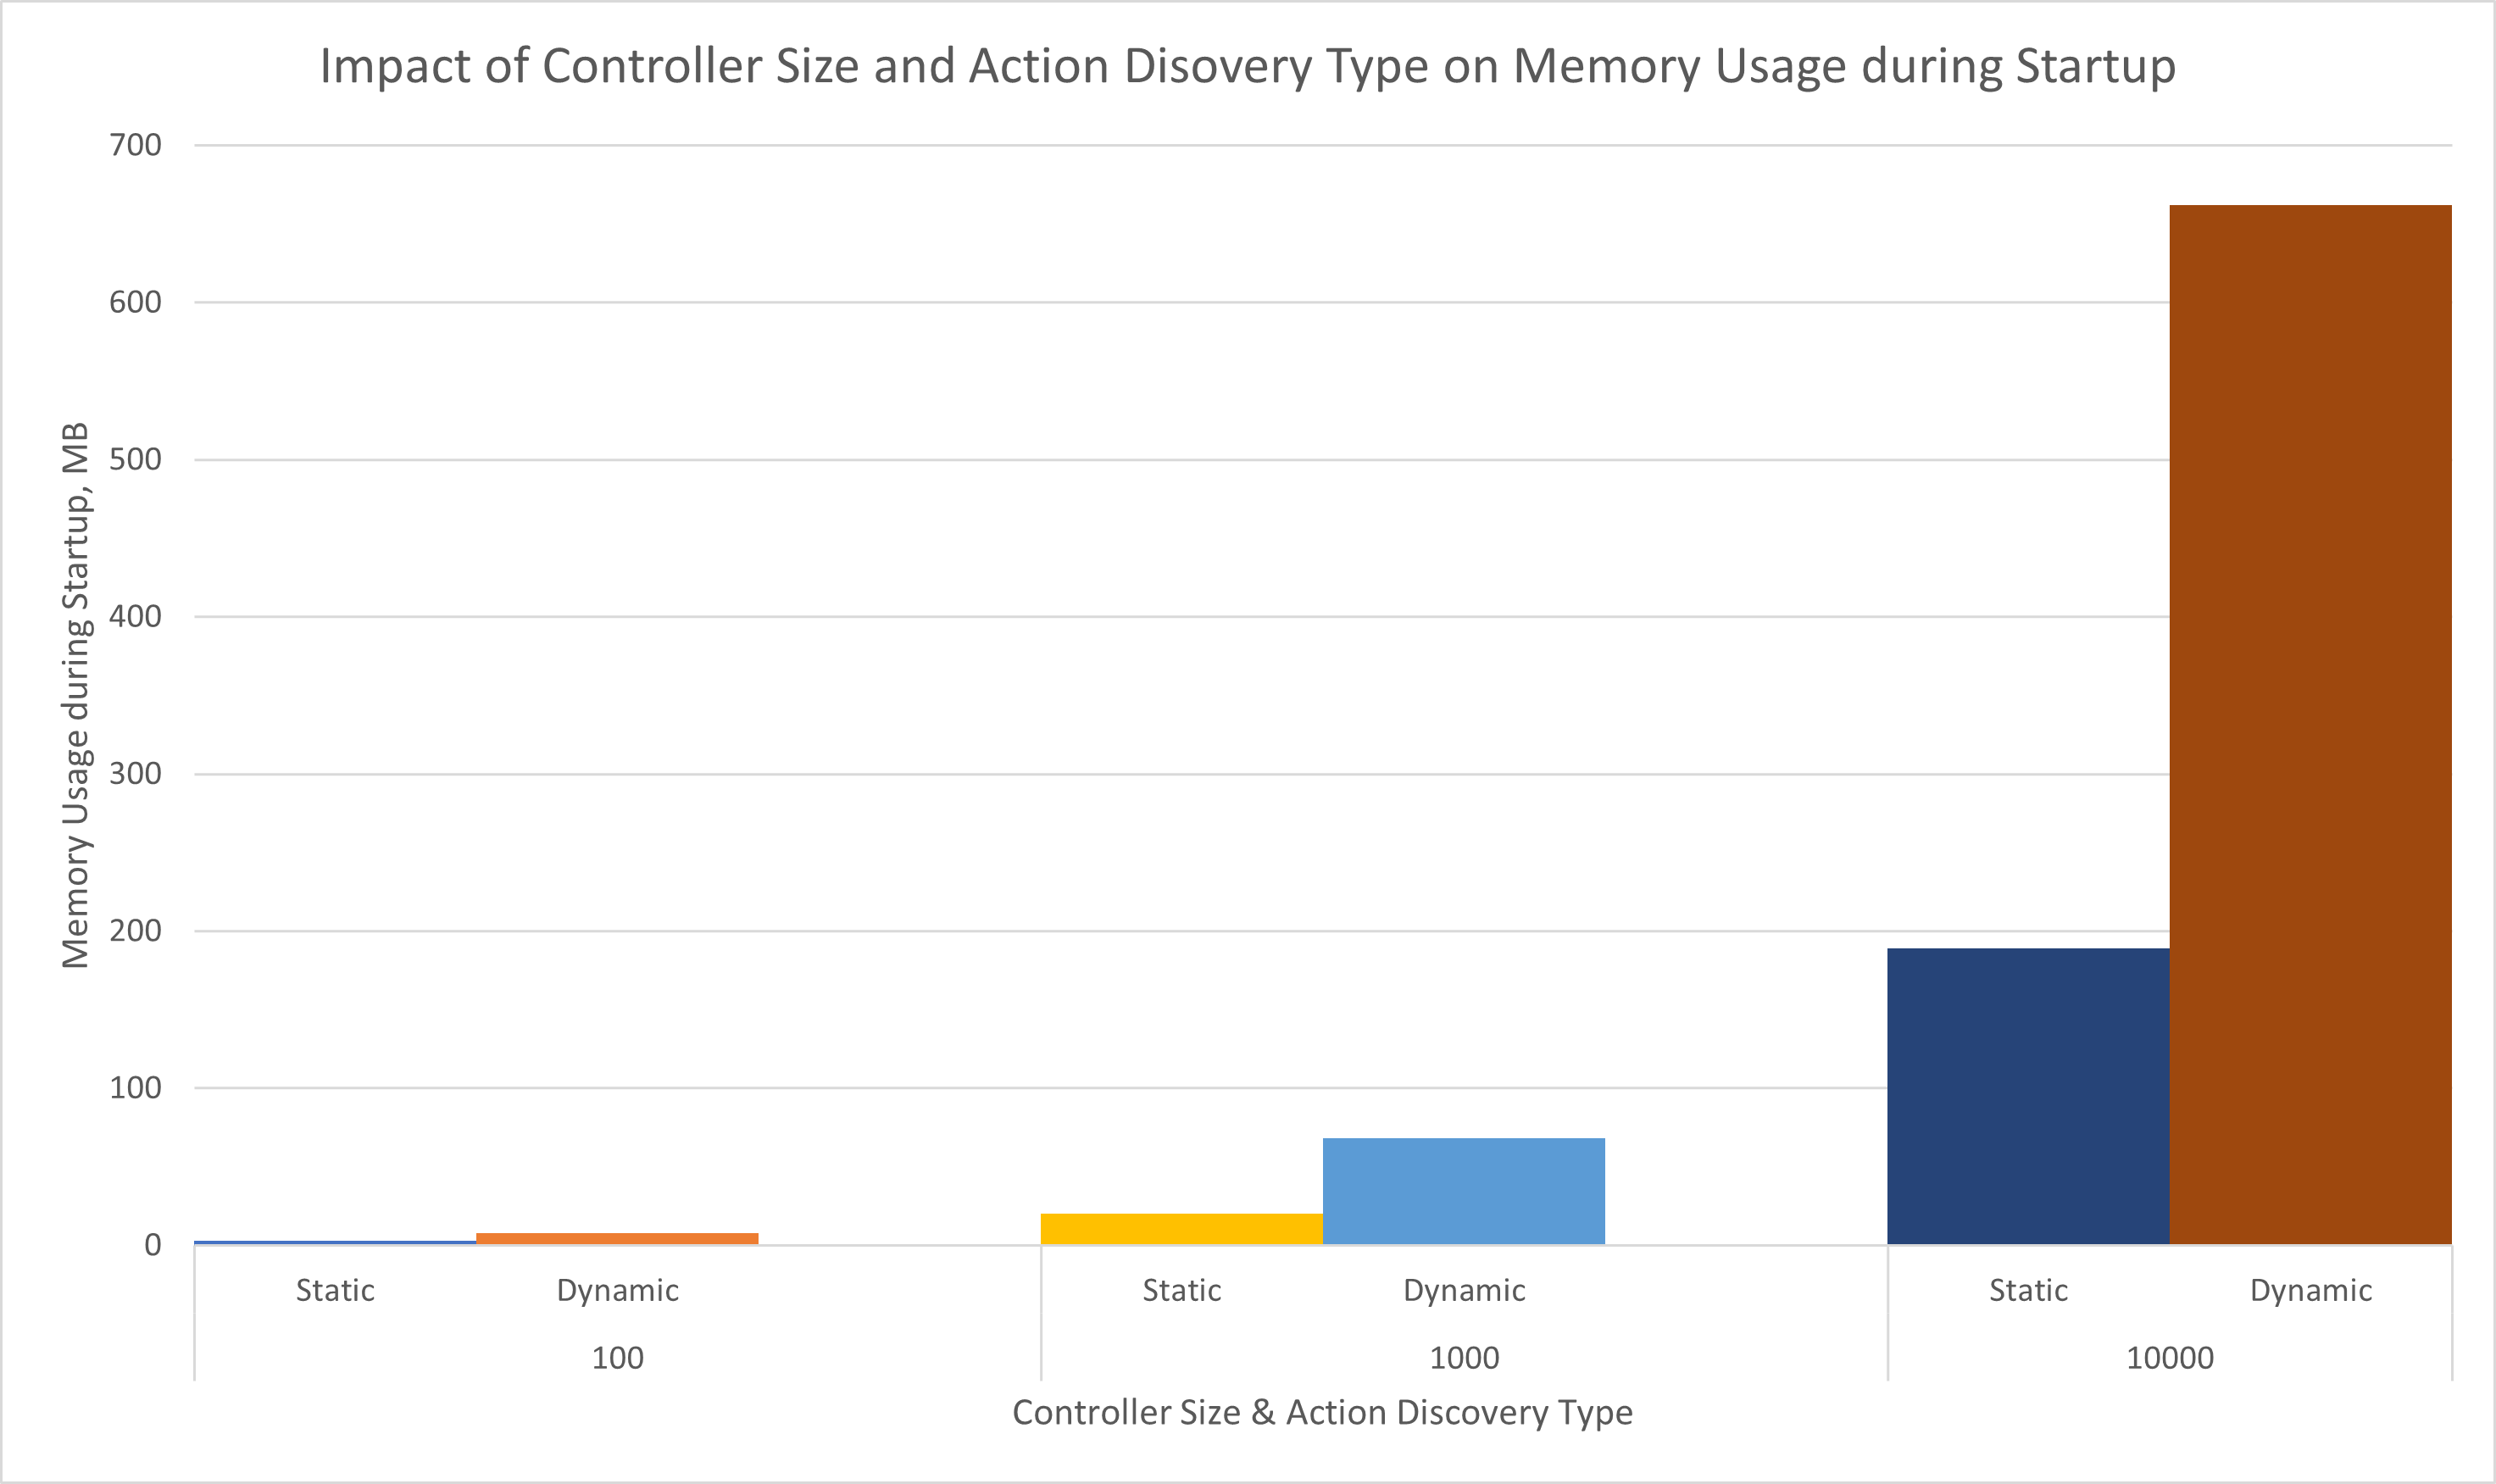
\includegraphics[width=0.8\textwidth]{graphics/Impact of Controller Size and Action Discovery Type on Memory Usage during Startup.png}
\caption{Impact of Controller Size and Action Discovery Type on Memory Usage during Startup}
\label{fig:memory-usage-results}
\end{figure}

A clear trend emerges from the data - the memory usage consistently increases in line with the number of controllers in an application. Specifically, the smallest application, consisting of 100 controllers, consumes 3 Megabytes (MB) of memory using static action discovery, while the dynamic approach uses more than double, at 8 MB.

Moving to the medium-sized application with 1,000 controllers, memory usage increases to 20 MB for the static method, while the dynamic counterpart demonstrates an even greater increase, reaching 68 MB.

Finally, the largest application of 10,000 controllers exhibits substantial memory usage: 189 MB for the static action discovery approach and a notably higher 662 MB for the dynamic method.